\section{问题二模型的建立与求解}

\subsection{数据处理与建模思路}

问题二与问题一相比，微网物理结构没有变化，最大的不同在于每天 0:00 制定计划时无法提前知道当天真实负荷和真实光伏。若全天计划不足，则需要按照交易时刻电价的 5 倍进行紧急购电。因此，问题二必须区分“0:00 事前计划”和“实际运行后的物理执行”。

问题一中已经建立了 \(G^L,G^{ch},PV^{ch},C,D,E,V,u\) 组成的能量分流物理模型。问题二继续沿用这组变量，但这些物理执行变量不应在 0:00 全部锁死。题目真正要求提前确定的是全天计划购电量，因此增加第一阶段变量 \(G^{plan}_{d,t}\)， 表示日期 \(d\) 在 0:00 对第 \(t\) 个 10 min 时段提交的正常计划购电功率。

实际负荷和光伏实现后，如果计划电和储能仍无法满足负荷，则需要紧急购电，因此增加 \(H_{d,t}\)， 表示紧急购电功率。

另一方面，计划购电已经在 0:00 确定并按计划量计费，当实际负荷低于预测、储能又无法继续吸收时，计划电中可能有一部分无法利用，因此增加 \(W_{d,t}\)， 表示已购未用电功率。由此，问题二的变量沿用问题一的物理变量，只在题目的计划机制下自然增加 \(G^{plan},H,W\)。

每天仍划分为 \(T=144,\qquad \Delta t=\frac16\ \mathrm{h}\)。 2025 年 1 月作为已知数据预热期，直接使用真实负荷和真实光伏建立预测历史；正式滚动规划从 2025 年 2 月 1 日开始。

储能参数保持

\[
1200\le E_{d,t}\le10800,
\]

\[
0\le C_{d,t},D_{d,t}\le5000,
\]

\[
\eta_c=\eta_d=0.90.
\]

问题二不再要求每天首末储电量相同，而采用跨日连续：

\begin{equation}
E^{act}_{d+1,0}=E^{act}_{d,T}.
\end{equation}

\subsection{完美信息确定性基准模型}

为衡量预测不确定性本身带来的额外成本，先建立逐日完美信息基准：假设每天 0:00 已知当天真实负荷与光伏，
则在问题一模型上增加紧急购电变量 \(H\)。光伏直供量与富余量由真实数据直接构造
（\(\overline L_{d,t}=\max(L_{d,t}-PV_{d,t},0)\)、\(\overline{PV}_{d,t}=\max(PV_{d,t}-L_{d,t},0)\)），
负荷平衡、充电来源、光伏剩余平衡、储能状态递推、容量与功率限制、充放电互斥的形式
均与问题一相同，只是负荷平衡中增加 \(H_{d,t}\)：

\begin{equation}
G^L_{d,t}+D_{d,t}+H_{d,t}=\overline L_{d,t},
\qquad
PV^{ch}_{d,t}+G^{ch}_{d,t}=C_{d,t},
\qquad
PV^{ch}_{d,t}+V_{d,t}=\overline{PV}_{d,t}.
\end{equation}

该基准在已知真实数据的条件下求全天费用最小，构成预测不确定性成本的下界。

\subsection{预测模型与 SAA 情景生成}

每天 \(d\) 只使用 \(d\) 日以前已经发生的历史真实数据建立负荷和光伏中心预测，记为 \(\hat L_{\tau,t}^{(d)},
\qquad
\widehat{PV}_{\tau,t}^{(d)}\)。 在基础点预测上保留偏差校正，以降低系统性供电不足风险。

对历史日期 \(r\)，定义负荷和光伏预测误差

\[
e^L_{r,t}
=
L_{r,t}^{act}
-
\hat L_{r,t},
\]

\begin{equation}
e^{PV}_{r,t}
=
PV_{r,t}^{act}
-
\widehat{PV}_{r,t}.
\end{equation}

每个历史日保留完整的 144 槽误差向量，负荷误差与光伏误差尽量从同一历史日期联合抽取，不逐槽独立打乱。

正式模型保留最近 28 个有效历史残差日，并随机无放回抽取 \(K=4\) 个完整误差日，随机种子固定为 2026。

第 \(\omega\) 个情景为

\begin{equation}
L_{\tau,t}^{(\omega)}
=
\max
\left\{
0,
\hat L_{\tau,t}^{(d)}
+
e^L_{r_\omega,t}
\right\},
\end{equation}

\begin{equation}
PV_{\tau,t}^{(\omega)}
=
\max
\left\{
0,
\widehat{PV}_{\tau,t}^{(d)}
+
e^{PV}_{r_\omega,t}
\right\}.
\end{equation}

SAA 的作用是用有限个历史误差情景近似未来预测误差分布，使 0:00 的计划购电能够提前考虑 5 倍紧急购电风险。

\subsection{7 日滚动视野}

若仅优化当天，模型容易在当天结束前大量放电，从而忽略剩余储电量对未来日期的价值。为减小该末端效应，每天 \(d\) 的 0:00 同时优化 \(d,d+1,\ldots,d+6\) 共 7 天，但只真正执行第 1 天。

后 6 天的计划变量仅用于估计当前日末储电量的未来延续成本，并不代表今天提前提交未来日期的正式购电计划。

由此取滚动视野

\[
R=7.
\]

\subsection{随机情景下的物理约束}

物理约束与问题一逐条对应，只是全部带上情景标号。光伏直供量与富余量仍由情景数据直接构造：
\(\overline L^{(\omega)}_{\tau,t}=\max(L^{(\omega)}_{\tau,t}-PV^{(\omega)}_{\tau,t},0)\)、
\(\overline{PV}^{(\omega)}_{\tau,t}=\max(PV^{(\omega)}_{\tau,t}-L^{(\omega)}_{\tau,t},0)\)。
三类能量流向平衡相应写为

\begin{equation}
G^{L,(\omega)}_{\tau,t}+D^{(\omega)}_{\tau,t}+H^{(\omega)}_{\tau,t}=\overline L^{(\omega)}_{\tau,t},
\qquad
PV^{ch,(\omega)}_{\tau,t}+G^{ch,(\omega)}_{\tau,t}=C^{(\omega)}_{\tau,t},
\qquad
PV^{ch,(\omega)}_{\tau,t}+V^{(\omega)}_{\tau,t}=\overline{PV}^{(\omega)}_{\tau,t},
\end{equation}

其中紧急购电 \(H\) 只用于补足负荷，不用于储能充电。储能递推、储电量上下限、充放电功率限制
与充放电互斥约束的形式与问题一完全相同，仅在每个情景内各自成立。此外，每个滚动日开始时的
储电量以当天真实值为准，所有情景共享同一初值：

\begin{equation}
E^{(\omega)}_{d,0}=E^{act}_{d,0}.
\end{equation}

\subsection{目标函数}

每天 \(d\) 的正式随机优化目标为

\begin{equation}
\min Z_d
=
C_d^{first}
+
\frac1K
\sum_{\omega=1}^{K}
Q_d^{(\omega)}.
\end{equation}

其中第一阶段全天计划购电费用为

\begin{equation}
C_d^{first}
=
\sum_t
\pi_tG^{plan}_{d,t}\Delta t.
\end{equation}

情景 \(\omega\) 下的补救及未来延续成本为

\begin{equation}
Q_d^{(\omega)}
=
\sum_t
5\pi_tH_{d,t}^{(\omega)}\Delta t
+
\sum_{\tau=d+1}^{d+6}\sum_t
\left[
\pi_tG_{\tau,t}^{plan,(\omega)}
+
5\pi_tH_{\tau,t}^{(\omega)}
\right]\Delta t.
\end{equation}

由此，模型在 0:00 同时权衡

\[
\boxed{
\text{提前正常购电成本}
\quad\longleftrightarrow\quad
\text{未来 5 倍紧急购电风险}
}
\]

并通过 7 日延续成本保留储能的跨日价值。

\subsection{实际执行规则}

0:00 求得当天 \(G^{plan}_{d,1:144}\) 后，计划在当天不再修改。

真实运行时依次执行：

\begin{enumerate}
\item 实际光伏优先满足负荷；
\item 当前计划购电补充负荷；
\item 仍不足时储能放电；
\item 储能仍不足时紧急购电；
\item 负荷满足后，富余光伏优先充电；
\item 再利用剩余计划电给储能充电；
\item 剩余光伏记为 \(V\)；
\item 剩余已购正常电记为 \(W\)；
\item 同一时段不得同时充放电。
\end{enumerate}

真实储电量按

\begin{equation}
E^{act}_{d,t}
=
E^{act}_{d,t-1}
+
0.9C^{act}_{d,t}\Delta t
-
\frac{D^{act}_{d,t}\Delta t}{0.9}
\end{equation}

更新，并将 \(E^{act}_{d+1,0}
=
E^{act}_{d,T}\) 传递至下一滚动日。

\subsection{模型求解}

经 SAA 情景展开后，模型的目标函数和能量平衡、储能递推、计划连接等约束均为线性形式，同时存在充放电状态二元变量 \(u\)，因此确定性等价模型属于混合整数线性规划。

采用分支定界/分支切割方法求解，并使用 MATLAB \texttt{intlinprog} 实现。首先放松整数约束求解 LP 松弛问题，并利用 LP 解进行热启动；随后对非整数状态变量进行分支，计算各节点下界，利用不可行剪枝和界剪枝排除不可能优于当前整数解的节点，同时使用切平面进一步收紧可行域。

每天的计算流程为：读取截至第 $d-1$ 日的历史数据，据此预测未来 7 日负荷与光伏，更新最近 28 个有效残差日并抽取 $K=4$ 个联合误差情景，构建 7 日滚动两阶段 SAA-MILP，经 LP 松弛热启动后用分支定界/分支切割求解，提取当天计划购电量，再按真实数据执行并更新储电量，随后进入下一滚动日。
全部算例正常收敛，最大约束违反约为 \(4.07\times10^{-8}\)， 最大绝对最优间隙约为 \(8.69\times10^{-4}\ \mathrm{元}\)， 相对于全年总费用数值上可视为 0。

\subsection{求解结果与结果分析}

正式报送窗口为 2025 年 2 月 1 日至 12 月 31 日。

全天计划购电费用为 \(13\,149\,064.98\ \mathrm{元}\)， 紧急购电费用为 \(1\,657\,825.30\ \mathrm{元}\)， 总购电费用为 \(\boxed{
14\,806\,890.28\ \mathrm{元}
}\)。 累计紧急购电量为 \(269\,240.9\ \mathrm{kWh}\)。 334 个报送日中，共有 175 天发生紧急购电，紧急购电时段共 1342 个，最大单个 10 min 时段紧急购电量为 966.770 kWh。

报送窗口日末储电量统计为

\[
\text{mean}=7046.0,
\qquad
\text{median}=8058.5,
\]

\[
\min=1200,
\qquad
\max=10800\ {\rm kWh}.
\]

四个指定日期结果如下：

\begin{table}[H]
\centering
\zihao{5}
\begin{tabular}{lrrrr}
\toprule
日期 & 日费用/元 & 紧急购电量/kWh & 日末储电量/kWh & 计划购电总量/kWh \\
\midrule
2025-03-20 & 41535.92 & 0.00 & 4077.0 & 66288.5 \\
2025-06-21 & 20827.44 & 0.00 & 8313.3 & 38911.0 \\
2025-09-23 & 71204.80 & 5351.69 & 5624.4 & 60974.9 \\
2025-12-21 & 66180.88 & 0.00 & 9391.2 & 101929.1 \\
\bottomrule
\end{tabular}
\caption{问题二典型日逐日指标（费用单位：元，电量单位：kWh）}
\label{tab:7}
\end{table}

%FIG:BEGIN q2-year
报送窗口内逐日的购电结构见图~\ref{fig:q2-year}。

\begin{figure}[htbp]
\centering
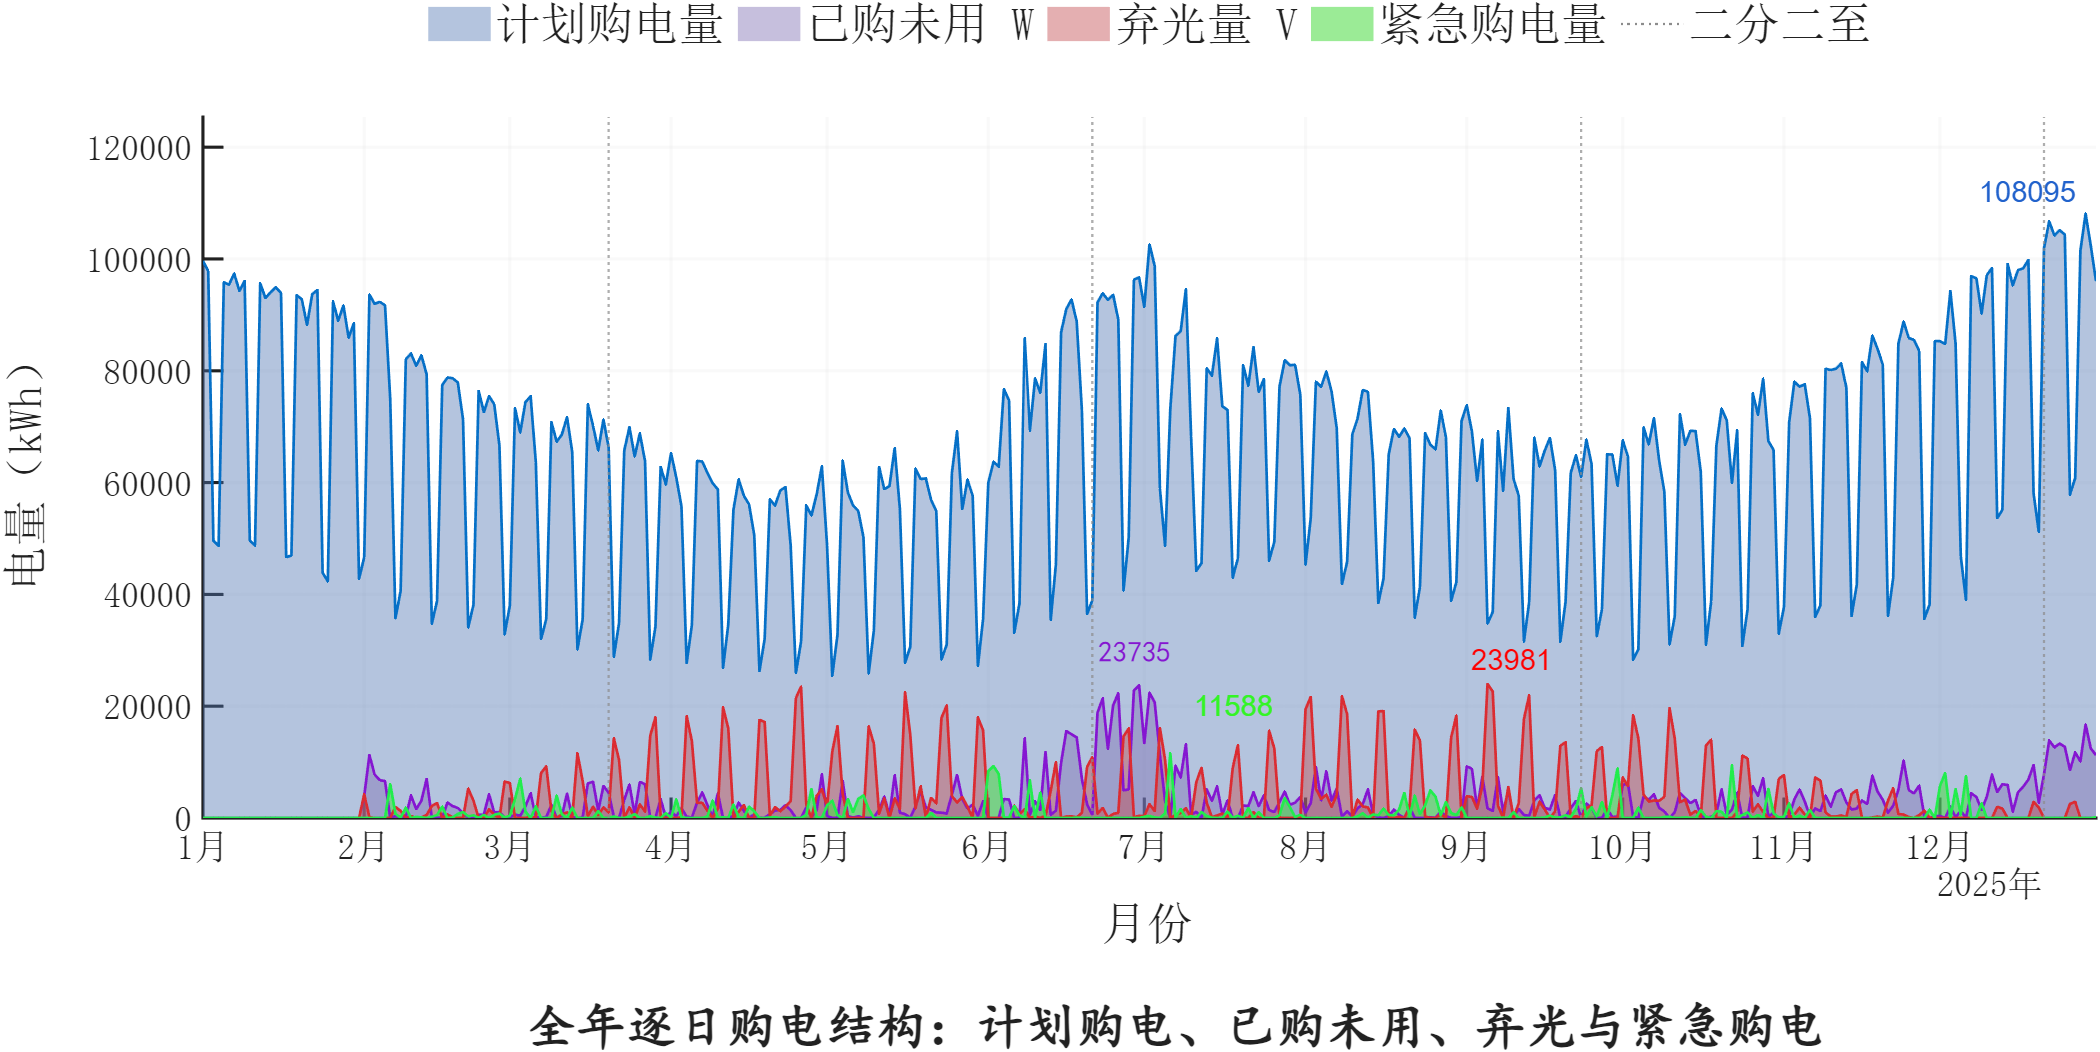
\includegraphics[width=0.78\textwidth,height=0.26\textheight,keepaspectratio]{figures/q2_year.png}
\caption{报送窗口内逐日购电结构（电量单位：kWh）}
\label{fig:q2-year}
\end{figure}

计划购电逐日平稳且季节性强，弃光、已购未用与紧急购电三者的量级都远小于计划购电，其峰值集中在夏秋两季。
%FIG:END q2-year

%FIG:BEGIN q2-soc
日末储电量的全年轨迹见图~\ref{fig:q2-soc}。

\begin{figure}[htbp]
\centering
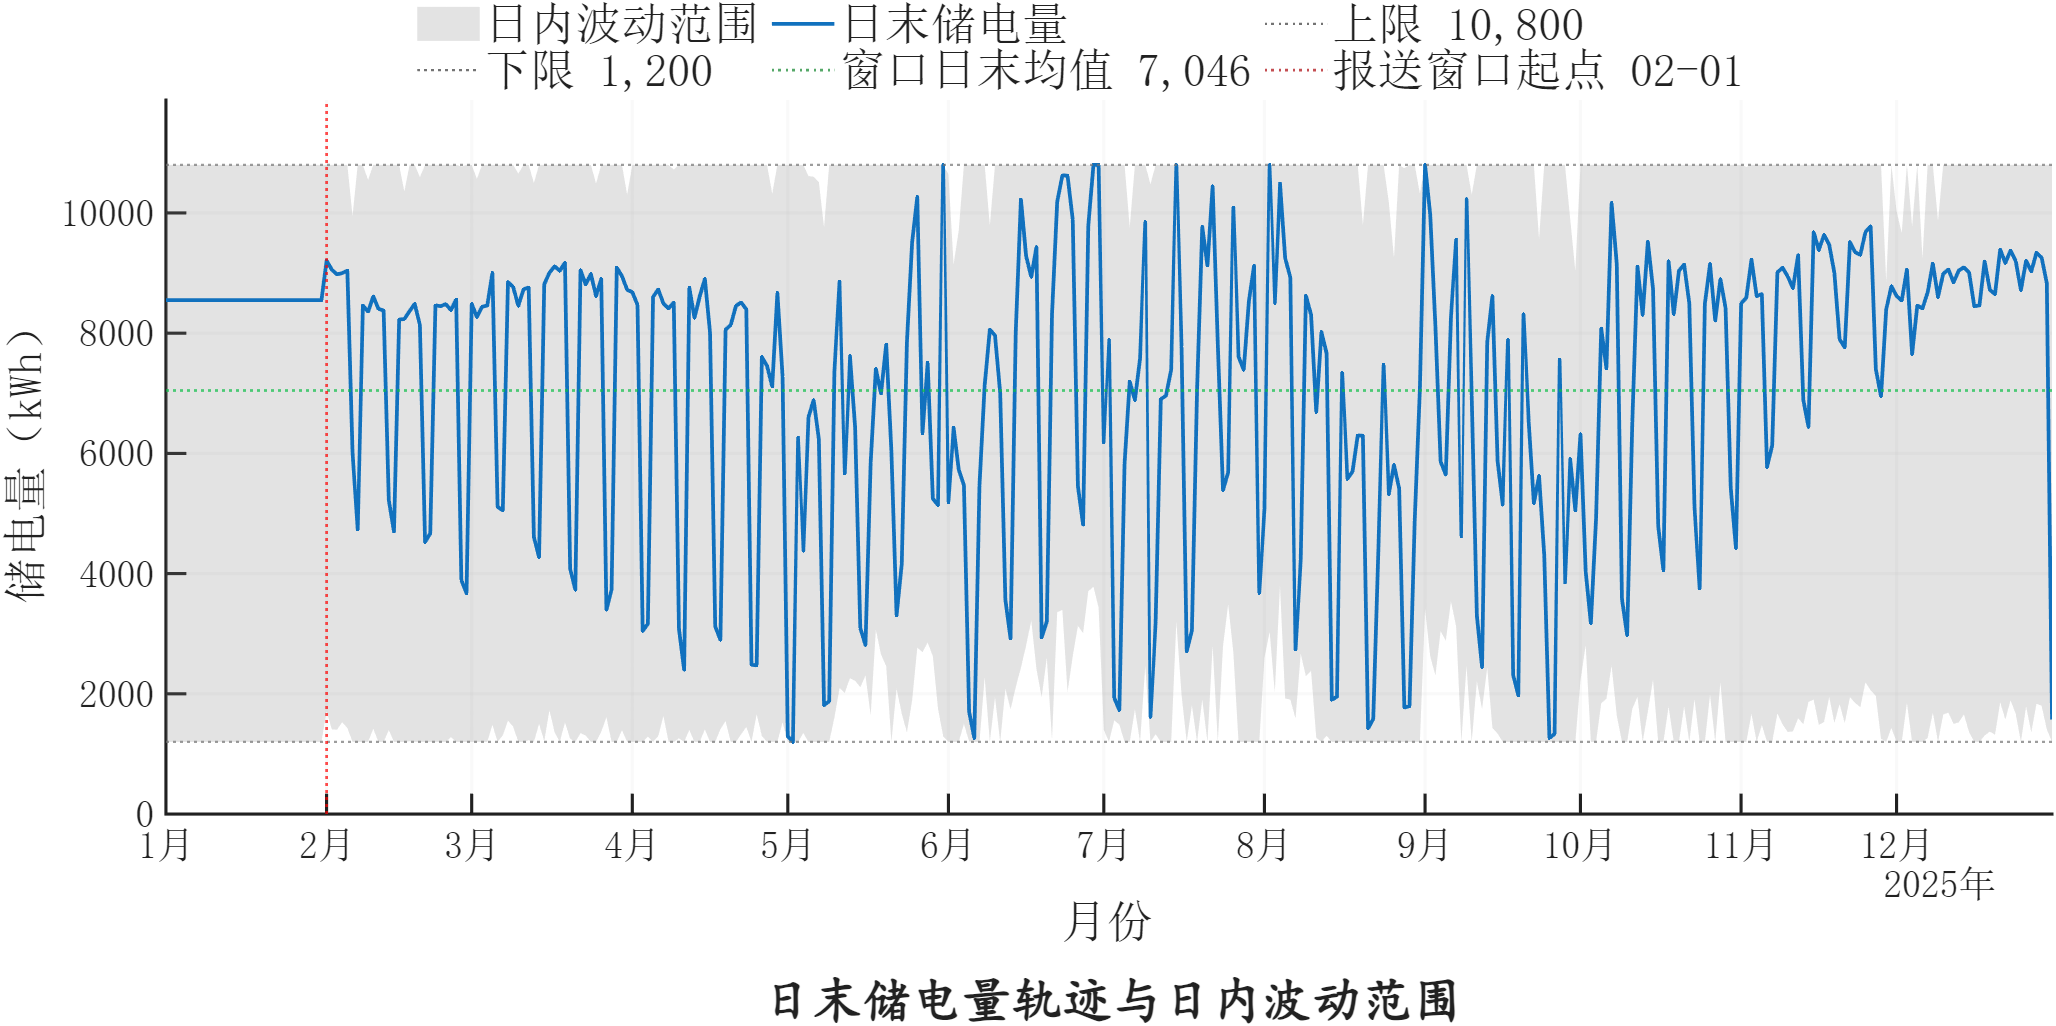
\includegraphics[width=0.78\textwidth,height=0.26\textheight,keepaspectratio]{figures/q2_soc.png}
\caption{问题二报送窗口内日末储电量轨迹（电量单位：kWh）}
\label{fig:q2-soc}
\end{figure}

报送窗口内日末储电量均值为 7\,046 kWh，全年仅 1 天触到 1\,200 kWh 的下限，说明 7 日滚动视野的终端价值设定有效，日末储电量没有被放空。
%FIG:END q2-soc
%MANDATED:BEGIN
按题目表 1、表 2 与表 3 要求的格式，四个指定日期的结果整理见后续横版页。

{\zihao{6}\setlength{\tabcolsep}{2pt}
\begin{center}
\begin{tabular}{|c|r|c|r|c|r|}
\hline
时间段 & 购电量/kWh & 时间段 & 购电量/kWh & 时间段 & 购电量/kWh \\
\hline
10:00-10:10 & \textbf{0.00} & 12:00-12:10 & \textbf{730.72} & 14:00-14:10 & \textbf{0.00} \\
\hline
16:00-16:10 & \textbf{507.64} & 18:00-18:10 & \textbf{690.59} & 20:00-20:10 & \textbf{0.00} \\
\hline
全天购电量 & \textbf{66288.55} & & & 全天购电费 & \textbf{41535.92} \\
\hline
\end{tabular}
\par{\zihao{6}表 1（2025.3.20）　问题二}

\vspace{0.15\baselineskip}
\begin{tabular}{|c|r|r|c|r|r|}
\hline
时间段 & 充电量/kWh & 放电量/kWh & 时间段 & 充电量/kWh & 放电量/kWh \\
\hline
0:00-4:00 & \textbf{1209.39} & \textbf{346.66} & 4:00-8:00 & \textbf{1641.51} & \textbf{4545.26} \\
\hline
8:00-12:00 & \textbf{5458.12} & \textbf{3265.56} & 12:00-16:00 & \textbf{3881.82} & \textbf{259.22} \\
\hline
16:00-20:00 & \textbf{180.35} & \textbf{5075.92} & 20:00-24:00 & \textbf{3173.35} & \textbf{3686.76} \\
\hline
0:00 储电量 & \textbf{9175.12} & & 24:00 储电量 & \textbf{4077.01} & \\
\hline
\end{tabular}
\par{\zihao{6}表 2（2025.3.20）　问题二}

\vspace{0.15\baselineskip}
\begin{tabular}{|c|r|c|r|c|r|}
\hline
时间段 & 购电量/kWh & 时间段 & 购电量/kWh & 时间段 & 购电量/kWh \\
\hline
10:00-10:10 & \textbf{0.00} & 12:00-12:10 & \textbf{0.00} & 14:00-14:10 & \textbf{0.00} \\
\hline
16:00-16:10 & \textbf{68.68} & 18:00-18:10 & \textbf{318.42} & 20:00-20:10 & \textbf{0.00} \\
\hline
全天购电量 & \textbf{38911.04} & & & 全天购电费 & \textbf{20827.44} \\
\hline
\end{tabular}
\par{\zihao{6}表 1（2025.6.21）　问题二}

\vspace{0.15\baselineskip}
\begin{tabular}{|c|r|r|c|r|r|}
\hline
时间段 & 充电量/kWh & 放电量/kWh & 时间段 & 充电量/kWh & 放电量/kWh \\
\hline
0:00-4:00 & \textbf{310.78} & \textbf{348.09} & 4:00-8:00 & \textbf{788.78} & \textbf{1724.85} \\
\hline
8:00-12:00 & \textbf{9897.19} & \textbf{0.00} & 12:00-16:00 & \textbf{0.00} & \textbf{0.00} \\
\hline
16:00-20:00 & \textbf{0.00} & \textbf{5584.97} & 20:00-24:00 & \textbf{7987.49} & \textbf{3122.97} \\
\hline
0:00 储电量 & \textbf{3206.20} & & 24:00 储电量 & \textbf{8313.25} & \\
\hline
\end{tabular}
\par{\zihao{6}表 2（2025.6.21）　问题二}

\vspace{0.15\baselineskip}
\begin{tabular}{|c|r|c|r|c|r|}
\hline
时间段 & 购电量/kWh & 时间段 & 购电量/kWh & 时间段 & 购电量/kWh \\
\hline
10:00-10:10 & \textbf{0.00} & 12:00-12:10 & \textbf{330.01} & 14:00-14:10 & \textbf{0.00} \\
\hline
16:00-16:10 & \textbf{424.60} & 18:00-18:10 & \textbf{595.42} & 20:00-20:10 & \textbf{0.00} \\
\hline
全天购电量 & \textbf{60974.88} & & & 全天购电费 & \textbf{71204.80} \\
\hline
\end{tabular}
\par{\zihao{6}表 1（2025.9.23）　问题二}

\vspace{0.15\baselineskip}
\begin{tabular}{|c|r|r|c|r|r|}
\hline
时间段 & 充电量/kWh & 放电量/kWh & 时间段 & 充电量/kWh & 放电量/kWh \\
\hline
0:00-4:00 & \textbf{5158.75} & \textbf{805.22} & 4:00-8:00 & \textbf{850.99} & \textbf{6502.94} \\
\hline
8:00-12:00 & \textbf{2242.72} & \textbf{1140.14} & 12:00-16:00 & \textbf{6336.46} & \textbf{682.05} \\
\hline
16:00-20:00 & \textbf{11.54} & \textbf{6273.05} & 20:00-24:00 & \textbf{4918.46} & \textbf{2.00} \\
\hline
0:00 储电量 & \textbf{5174.47} & & 24:00 储电量 & \textbf{5624.39} & \\
\hline
\end{tabular}
\par{\zihao{6}表 2（2025.9.23）　问题二}

\vspace{0.15\baselineskip}
\begin{tabular}{|c|r|c|r|c|r|}
\hline
时间段 & 购电量/kWh & 时间段 & 购电量/kWh & 时间段 & 购电量/kWh \\
\hline
10:00-10:10 & \textbf{0.00} & 12:00-12:10 & \textbf{970.04} & 14:00-14:10 & \textbf{0.00} \\
\hline
16:00-16:10 & \textbf{847.50} & 18:00-18:10 & \textbf{719.18} & 20:00-20:10 & \textbf{0.00} \\
\hline
全天购电量 & \textbf{101929.11} & & & 全天购电费 & \textbf{66180.88} \\
\hline
\end{tabular}
\par{\zihao{6}表 1（2025.12.21）　问题二}

\vspace{0.15\baselineskip}
\begin{tabular}{|c|r|r|c|r|r|}
\hline
时间段 & 充电量/kWh & 放电量/kWh & 时间段 & 充电量/kWh & 放电量/kWh \\
\hline
0:00-4:00 & \textbf{2366.13} & \textbf{100.62} & 4:00-8:00 & \textbf{929.13} & \textbf{633.41} \\
\hline
8:00-12:00 & \textbf{5251.08} & \textbf{7197.13} & 12:00-16:00 & \textbf{6329.48} & \textbf{2183.12} \\
\hline
16:00-20:00 & \textbf{49.51} & \textbf{4461.69} & 20:00-24:00 & \textbf{8405.67} & \textbf{3654.96} \\
\hline
0:00 储电量 & \textbf{8649.86} & & 24:00 储电量 & \textbf{9391.17} & \\
\hline
\end{tabular}
\par{\zihao{6}表 2（2025.12.21）　问题二}

\vspace{0.15\baselineskip}
\begin{tabular}{|c|r|c|r|c|r|c|r|}
\hline
\multicolumn{2}{c|}{2025.3.20} & \multicolumn{2}{c|}{2025.6.21} & \multicolumn{2}{c|}{2025.9.23} & \multicolumn{2}{c|}{2025.12.21} \\
\hline
时间段 & 购电量/kWh & 时间段 & 购电量/kWh & 时间段 & 购电量/kWh & 时间段 & 购电量/kWh \\
\hline
无 & \textbf{0.00} & 无 & \textbf{0.00} & 8:20-10:00 & \textbf{1247.80} & 无 & \textbf{0.00} \\
\hline
 &  &  &  & 19:50-22:00 & \textbf{4103.89} &  &  \\
\hline
\end{tabular}
\par{\zihao{6}表 3　微网在指定日期的紧急购电量（问题二）}

\end{center}
}


%MANDATED:END

%FIG:BEGIN q2-key
四个指定日期的计划购电与紧急购电见图~\ref{fig:q2-key}。

\begin{figure}[htbp]
\centering
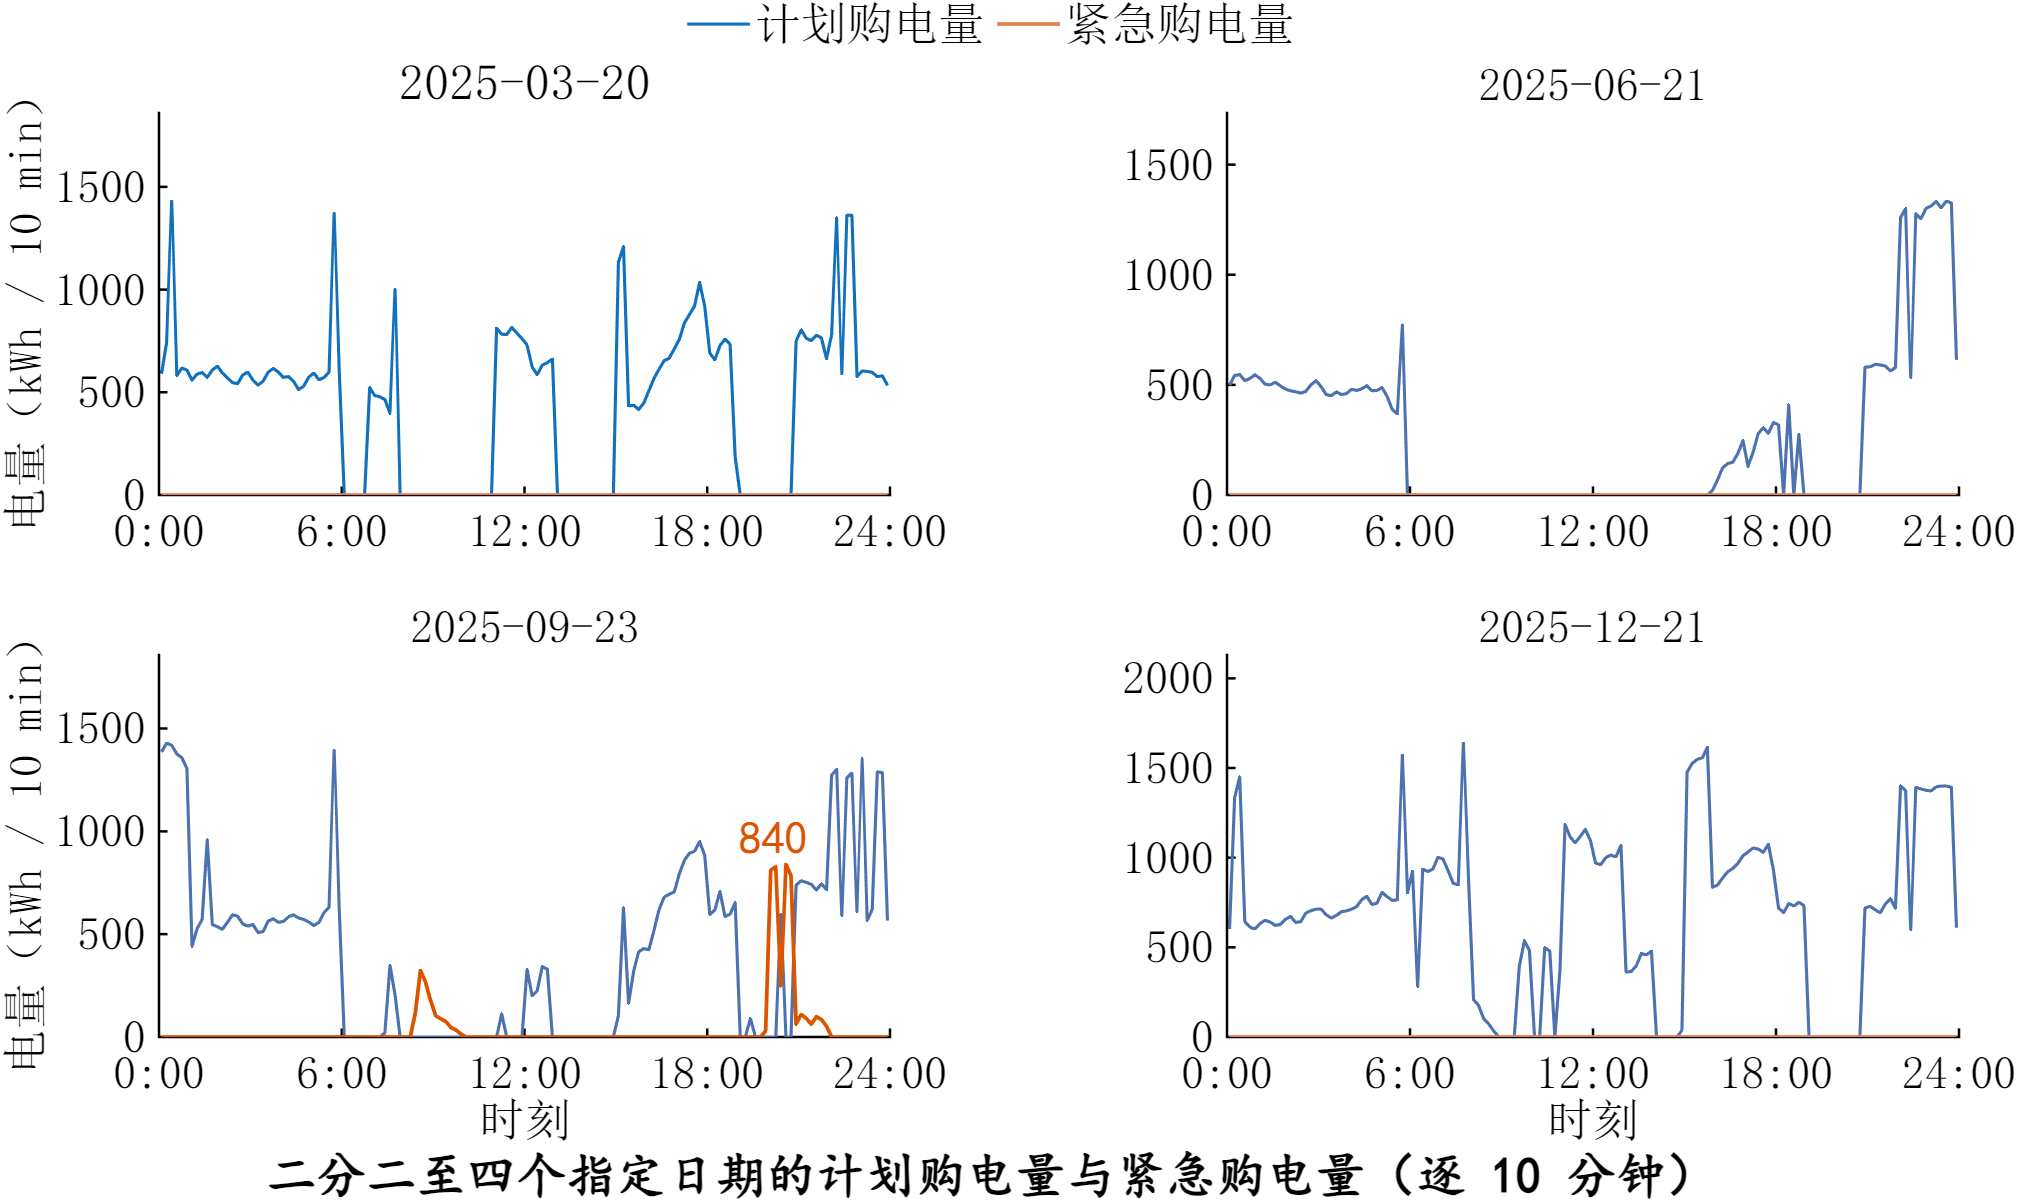
\includegraphics[width=0.78\textwidth,height=0.26\textheight,keepaspectratio]{figures/q2_keydate.png}
\caption{问题二四个指定日期的计划购电与紧急购电（电量单位：kWh）}
\label{fig:q2-key}
\end{figure}

四天中仅 09-23 触发紧急购电（5\,351.69 kWh，分 08:20—10:00 与 19:50—22:00 两段），其余三天均为零。
%FIG:END q2-key

为分析预测不确定性的成本，构造“全年联合完美信息—逐日完美信息—7 日滚动 SAA”三级信息集阶梯。三种模型对应费用分别为

\[
12\,227\,142.86\ {\rm 元},
\]

\[
12\,253\,936.65\ {\rm 元},
\]

\[
14\,806\,890.28\ {\rm 元}.
\]

因此正式随机模型相对于全年联合完美信息增加 \(2\,579\,747.42\ \mathrm{元}
=
257.97\ \mathrm{万元}\)。 其中，跨日/有限视野部分为

\[
12\,253\,936.65
-
12\,227\,142.86
=
26\,793.79\ {\rm 元}
=
2.68\ {\rm 万元},
\]

预测不确定性部分为

\[
14\,806\,890.28
-
12\,253\,936.65
=
2\,552\,953.63\ {\rm 元}
=
255.30\ {\rm 万元}.
\]

即

\[
\boxed{
257.97
=
2.68+255.30
\quad(\text{万元})
}
\]

说明问题二中成本上升的主要来源是负荷和光伏预测不确定性，而不是滚动视野不足。

\subsubsection{滚动视野分析}

当

\[
R=1,3,7
\]

时，总费用分别为 \(14\,884\,621.29,\quad
14\,806\,918.29,\quad
14\,806\,890.28\ \mathrm{元}\)， 日末平均储电量分别为 \(1961.4,\quad
7045.7,\quad
7046.0\ \mathrm{kWh}\)。 由 \(R=1\) 扩大至多日视野后，日末储电量明显恢复，说明多日滚动能够有效体现储能跨日价值；而 \(R=3\) 到 \(R=7\) 的边际费用改善已经很小。

\subsubsection{情景数稳定性}

当 \(K=4\) 时， \(Z=14\,806\,890.28\ \mathrm{元},
\qquad
Q_{em}=269\,240.9\ \mathrm{kWh}\)。 当 \(K=8\) 时，

\[
Z=14\,516\,318.96\ {\rm 元},
\qquad
Q_{em}=230\,031.1\ {\rm kWh}.
\]

总费用差异约 1.96\%，但紧急购电量差异约 14.56\%，说明费用对情景数相对稳定，而紧急购电风险对情景覆盖仍较敏感。

\subsubsection{偏差校正分析}

不带偏差校正时， \(14\,671\,204.28\ \mathrm{元},
\qquad
274\,289.2\ \mathrm{kWh}\)。 带偏差校正时， \(14\,806\,890.28\ \mathrm{元},
\qquad
269\,240.9\ \mathrm{kWh}\)。 即总费用增加约 0.92\%，紧急购电量下降约 1.8\%。因此偏差校正同时作用于经济性与供电可靠性，是两者之间的折中。